\documentclass{standalone}
\usepackage{tikz}
\usetikzlibrary{hobby}
\begin{document}
\newcommand\helpgrid[3]{ % args: x1 y1, step. The grid starts from (0,0) to (x1,y1) with given step
    \draw[help lines, color=gray, dashed] (0,0) grid[step={(#3,#3)}] (#1,#2);
    \foreach \x in {0,1,...,#1}
        {
            \node at (\x,0) {\textbf{\x}};
        }
    \foreach \y in {0,1,...,#2}
        {
            \node at (0,\y) {\textbf{\y}};
        }
}
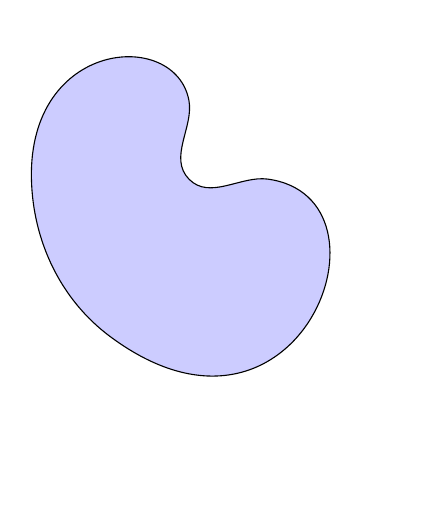
\begin{tikzpicture}
    \helpgrid{8}{8}{1}
    \path[draw,use Hobby shortcut,closed=true, fill=blue!20]
        (3, 2) .. (2, 4) .. (4, 5) .. (4, 4) .. (5, 4);
\end{tikzpicture}
\end{document}
